
\documentclass[12pt]{mitthesis}
\usepackage{titlesec}
\usepackage{geometry}
\usepackage{graphicx}
\usepackage{booktabs, chemformula}
\usepackage{titlesec, blindtext, color}
\usepackage{listings}
\usepackage{float}
\usepackage{xcolor} 
\usepackage{array}
\usepackage{color, colortbl}
\usepackage{caption}
\usepackage{amsmath}

\captionsetup{font=footnotesize}

\definecolor{lightgreen}{rgb}{0.82, 0.94, 0.75}
\definecolor{lightorange}{rgb}{0.98, 0.84, 0.65}
\newcolumntype{L}{>{\centering\arraybackslash}m{10cm}}
\newcolumntype{l}{>{\centering\arraybackslash}m{7cm}}
\def\BibTeX{{\rm B\kern-.05em{\sc i\kern-.025em b}\kern-.08em
    T\kern-.1667em\lower.7ex\hbox{E}\kern-.125emX}}

\newcommand*{\Comb}[2]{{}^{#1}C_{#2}}%

\pagestyle{plain}

\begin{document}

\title{Methods and Tools for the Analysis of Legacy Software Systems}

\author{Stana Adelina Diana}


\department{Department of Computers and Information Technology}


\thesisdate{Sept, 2019}


\supervisor{Vladimir Cretu}{Associate Professor}




\maketitle


\cleardoublepage

\setcounter{savepage}{\thepage}



\cleardoublepage



\tableofcontents

\pagestyle{plain}


\chapter{Introduction}


This report presents the results obtained so far on the proposed thesis. The goal of the thesis is to develop methods for analyzing legacy software systems, focusing on using historical information describing the evolution of the systems extracted from the versioning systems.

We have developed a tool that extracts and processes the needed information from a software system. The tool workflow and technologies used are presented in section \ref{sec:tool}. The primary information extracted by the tool is described in sections \ref{sec:sd_extraction} and \ref{sec:copairs_extraction}. The filtering methods selected to be applied to the extracted information are presented in sections \ref{sec:filtercommit}, \ref{sec:filterocc}, and \ref{sec:filterstrength}.

To perform measurements based on our assumptions, we have selected a set of 27 object-oriented software systems presented in section \ref{sec:dataset}. 
For each listed software system, the tool extracts, filters, and collects the information needed.

Each filtering section (\ref{sec:filtercommit}, \ref{sec:filterocc}, and \ref{sec:filterstrength}) contains the detailed results obtained after analyzing all the software systems and conclusions based on the results. 

Section \ref{sec:overlaps} focuses on the overlappings between the extracted information from the code and filtered information from the versioning systems. 

The conclusions and observations based on the performed measurements are presented in chapter \ref{conclusions}.




\chapter{Extracting software dependencies}
\label{extraction}

\section{Tool for measuring software dependencies}
\label{sec:tool}

To establish structural and logical dependencies, we developed a tool that takes as input the source code repository URL of a given system and extracts from it the software dependencies \cite{DepSACI}. 
From a workflow point of view, we can identify 3 major types of activities that the tool does: downloads the required data from the git repository, extracts from the source code the structural dependencies and, extracts and filters the co-changing pairs from the repository's commit history. Figure \ref{fig:figworkflow} represents the activities mentioned above. Each block represents a different activity. 

\begin{figure}[H]
\centering
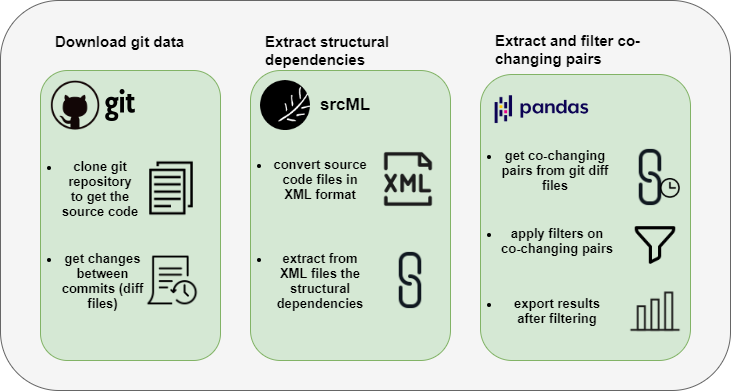
\includegraphics[width=\textwidth]{tool_workflow.png}
\caption{Tool workflow and major activities.}
\label{fig:figworkflow}
\end{figure}


\textbf{Download git data.}

The source code repository provides us all the needed information to extract both types of dependencies. It holds the code of the system but also the change history of the system. We use the source code for structural dependencies extraction \ref{sec:sd_extraction} and the change history for co-changing pairs extraction \ref{sec:copairs_extraction}.
To get the source code files and the change history, we first need to know the repository URL from GitHub (GitHub is a Git repository cloud-based hosting service). With the GitHub URL and a series of Git commands, the tool can download all the necessary data for dependencies extraction.

As we can see in figure \ref{fig:figgitdata}, the \textit{"clone"} command will download a Git repository to your local computer, including the source code files. The \textit{"diff"} command will get the differences between two existing commits in the Git repository. 
The tool gets the Git repository and the source code files by executing the "clone" command. Afterward, it gets all the existing commits within the Git repository. The commits are ordered by date, beginning with the oldest one and ending with the most recent one. The tool executes the "diff" command between each commit and its parent (the previous commit). The "diff" command generates a text file that contains the differences between the two commits: code differences, the number of files changed and changed file names.


\begin{figure}[H]
\centering
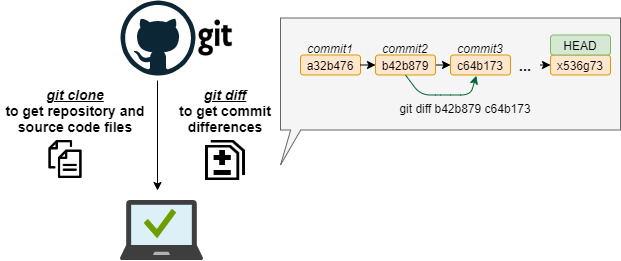
\includegraphics[width=\textwidth]{gitdata.png}
\caption{Commands used to download the required data from GitHub.}
\label{fig:figgitdata}
\end{figure}

\textbf{Extract structural dependencies.}

To extract the structural dependencies from the source code files the tool converts each source code file into srcML format using an open-source tool called srcML. The srcML format is an XML representation for source code. Each markup tag identifies elements of the abstract syntax for the language \cite{srcML}. 
After conversion, the tool parses each file and identifies all the defined entities (class, interface, enum, struct) within the file. It also identifies all the entities that are used by the entities defined.  The connection between both types of entities mentioned above constitutes a structural dependency.

\textbf{Extract and filter co-changing pairs.}

The process of extracting and filtering the co-changing pairs is represented in figure \ref{fig:figfiltering}.
For co-changing pairs extraction, the tool parses each generated diff file.
For each file, the tool gets the number of changed files and the name of the files. 
After structural dependencies extraction, the tool knows all the software entities contained in a file. Two entities from two changed files form a co-changing pair. After all the co-changing pairs of one diff file are extracted, the tool moves to the next diff file and extracts the set of co-changing pairs.

As presented in sections \ref{sec:filtercommit}, \ref{sec:filterocc}, and \ref{sec:filterstrength}, not every co-changing pair extracted is a logical dependency. For a co-changing pair to be labeled as a logical dependency, it has to meet some criteria. Each criterion constitutes a filter that a co-changing pair has to pass in order to be called logical dependency.
The filters are implemented in the tool and can be combined. The input for each filter is the set of co-changing pairs extracted, and the output is the remaining co-changing pairs that respect the filter criterion.


\begin{figure}[H]
\centering
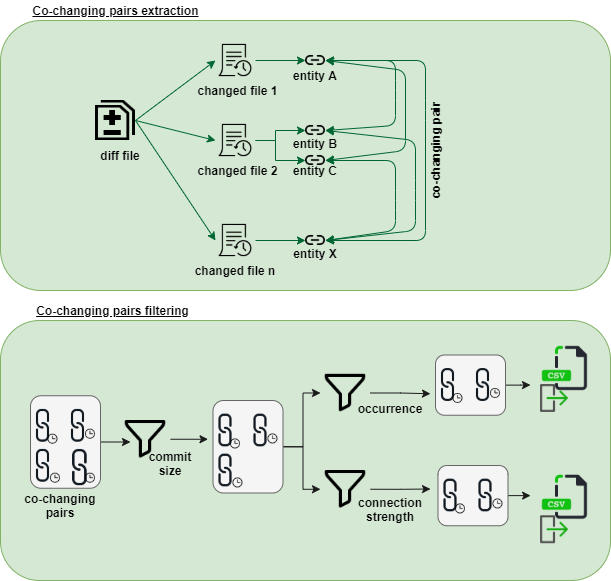
\includegraphics[width=\textwidth]{pairs_filtering.png}
\caption{Co-changing pairs extraction and filtering.}
\label{fig:figfiltering}
\end{figure}


\section{Extracting structural dependencies}
\label{sec:sd_extraction}
A dependency is created between two elements that are in a relationship and indicates that an element of the relationship, in some manner, depends on the other element of the relationship \cite{Booch:2004:OAD:975416}, \cite{Cataldo2009SoftwareDW}.

Structural dependencies can be found by analyzing the source code \cite{Sangal:2005:UDM:1094811.1094824}, \cite{CalloArias2011}, \cite{structdep}. A structural dependency between two classes A and B is given by the fact that A statically depends on B, meaning that A cannot be compiled without knowing about B. In object oriented systems, this dependency can be given by many types of relationships between the two classes: A extends B, A implements B, A has attributes of type B, A has methods which have type B in their signature, A uses local variables of type B, A calls methods of B.


 We use an external tool called srcML \cite{srcML} to convert all source code files from the current release into XML files. All the information about classes, methods, calls to other classes are extracted by parsing the XML files and building a dependency data structure \cite{2003:XLC:851042.857028},
\cite{Collard:2011:LTF:2067850.2068011}. We choose the srcML format because it has the same markup for different programming languages and can ease the parsing of source code written in various programming languages such as Java, C++, and C\#.


\section{Extracting co-changing pairs}
\label{sec:copairs_extraction}

\textit{Logical dependencies} (a.k.a logical coupling) can be found by software history analysis and can reveal relationships that are not always present in the source code (structural dependencies).  

Software engineering practice has shown that sometimes modules which do not present structural dependencies still can be related \cite{articleEvolution}. Co-evolution represents the phenomenon when one component changes in response to a change in another component \cite{Yu:2007:UCC:1231330.1231370}, \cite{5166450}. Those changes can be found in the software change history from the versioning system. Gall \cite{Gall:1998:DLC:850947.853338}, \cite{Gall:2003:CRH:942803.943741} identified as logical coupling between two modules the fact that these modules \textit{repeatedly} change together during the historical evolution of the software system \cite{6606615}.

The versioning system contains the long-term change history of every file. Each project change made by an individual at a certain point of time is contained into a commit \cite{7471284}. All the commits are stored in the versioning system chronologically and each commit has a parent. The parent commit is the baseline from which development began, the only exception to this rule is the first commit which has no parent \cite{svn}. 


Currently there is no set of rules or best practices that can be applied to the extracted class co-changes and can guarantee their filtering into a set of logical dependencies.


This is mainly because not all the updates made in the versioning system are code related. For example a commit that has as participants a big number of files can indicate that a merge with another branch or a folder renaming has been made. In this case, a series of irrelevant co-changing pairs of entities can be introduced. So, in order to exclude this kind of situations the information extracted from the versioning system has to be filtered first and then used. Surveys also show that historical information is rarely used due to the size of the extracted information \cite{Shtern:2012:CMS:2332427.2332428}, \cite{sar}.

Other works have tried to filter co-changes \cite{Oliva:2011:ISL:2067853.2068086}, \cite{DBLP:journals/jss/AjienkaC17}. One of the used co-changes filter is the commit size.The commit size is the number of code files changed in that particular commit. 
Ajienka and Capiluppi established a threshold of 10 for the maximum accepted size for a commit \cite{DBLP:journals/jss/AjienkaC17}. This means that all the commits that had more than 10 code files changed where discarded from the research. But setting a harcoded threshold for the commit size is debatable because in order to say that a commit is big or small you have to look first at the size of the system and at the trends from the versioning system. Even thought the best practices encourage small and often commits, the developers culture is the one that influences the most the trending size of commits from one system.

Filtering only after commit size is not enough, this type of filtering can indeed have an impact on the total number of extracted co-changes, but will only shrink the number of co-changes extracted without actually guaranteeing that the remaining ones have more relevancy and are more linked.

Although, some unrelated files can be updated by human error in small commits, for example: one file was forgot to be commited in the current commit and will be commited in the next one among some unrelated files. This kind of situation can introduce a set of co-changing pairs that are definitely not logical liked. In order to avoid this kind of situation a filter for the occurrence rate of co-changing pairs can be introduced. Co-changing pairs that occur multiple times are more prone to be logically dependent than the ones that occur only once. Currently there are no concrete examples of how the threshold for this type of filter can be calculated. In order to do that, incrementing the threshold by a certain step will be the start and then studying the impact on the remaining co-changing pairs for different systems. 

Nevertheless, logical dependencies should integrate harmoniously with structural dependencies in an unitary dependency model: valid logical dependencies should not be omitted from the dependency model, but structural dependencies should not be engulfed by questionable logical dependencies generated by casual co-changes.  
Thus, in order to add logical dependencies besides structural dependencies in dependency models, class co-changes must be filtered until they remain only a reduced but relevant set of valid logical dependencies. 



\chapter {Filtering extracted co-changing pairs}

\section{Data set used}
\label{sec:dataset}
We have analyzed a set of open-source projects found on GitHub\footnote{http://github.com/} \cite{Kalliamvakou2016} in order to extract the structural and logical dependencies between classes. Table \ref{table:1} enumerates all the systems studied. The 1st column assigns the projects IDs; 2nd column shows the project name; 3rd column shows the number of entities(classes and interfaces) extracted; 4th column shows the number of most recent commits analyzed from the active branch of each project and the 5th shows the language in which the project was developed.


\begin{table}[!h]
\renewcommand{\arraystretch}{1}
\caption{Summary of open source projects studied.}
\label{table:1}
\centering
\scalebox{0.9}{
\begin{tabular}{|c|c|c|c|c|c|}
\hline
   ID  & Project    & Nr. of & Nr. of& Type\\
     &     & entites & commits & \\
\hline
1	&	bluecove	&	2685	&	894	&	java	\\
2	&	aima-java	&	5232	&	1006	&	java	\\
3	&	powermock	&	2801	&	949	&	java	\\
4	&	restfb	&	3350	&	1391	&	java	\\
5	&	rxjava	&	21097	&	4398	&	java	\\
6	&	metro-jax-ws	&	6482	&	2927	&	java	\\
7	&	mockito	&	5189	&	3330	&	java	\\
8	&	grizzly	&	10687	&	3113	&	java	\\
9	&	shipkit	&	639	&	1563	&	java	\\
10	&	OpenClinica	&	9655	&	3276	&	java	\\
11	&	robolectric	&	8922	&	5912	&	java	\\
12	&	aeron	&	4159	&	5977	&	java	\\
13	&	antlr4	&	4747	&	4431	&	java	\\
14	&	mcidasv	&	3272	&	4136	&	java	\\
15	&	ShareX	&	4289	&	5485	&	csharp	\\
16	&	aspnetboilerplate	&	9712	&	4323	&	csharp	\\
17	&	orleans	&	16963	&	3995	&	csharp	\\
18	&	cli	&	2063	&	4488	&	csharp	\\
19	&	cake	&	12260	&	2518	&	csharp	\\
20	&	Avalonia	&	16732	&	5264	&	csharp	\\
21	&	EntityFrameworkCore	&	50179	&	5210	&	csharp	\\
22	&	jellyfin	&	8764	&	5433	&	csharp	\\
23	&	PowerShell	&	2405	&	3250	&	csharp	\\
24	&	WeiXinMPSDK	&	7075	&	5729	&	csharp	\\
25	&	ArchiSteamFarm	&	702	&	2497	&	csharp	\\
26	&	VisualStudio	&	4869	&	5039	&	csharp	\\
27	&	CppSharp	&	17060	&	4522	&	csharp	\\

\hline
\end{tabular}
}
\end{table}



\section{Filtering based on size of commit transactions}
\label{sec:filtercommit}

As presented in section \ref{sec:copairs_extraction}, according to surveys,  co-changing pairs are not used because of their size. One system can have millions of co-changing pairs.
Whit this filtering type, we not only want to decrease the total size of the extracted co-changing pairs. But also to be one step closer to the identification of the logical dependencies among the co-changing pairs.
In this step, we want to filter the co-changing pairs extracted after commit size (cs). This means that the co-changing pairs are extracted only from commits that involve fewer files than an establised threshold number. 

Different works have chosen fixed threshold values for the maximum number of files accepted in a commit. Cappiluppi and Ajienka, in their works \cite{DBLP:journals/jss/AjienkaC17}, \cite{DBLP:journals/ese/AjienkaCC18} only take into consideration commits with less then 10 source code files changed in building the logical dependencies.

The research of Beck et al \cite{Beck:2011:CMC:2025113.2025162} only takes in consideration transactions with up to 25 files. The research \cite{Oliva:2011:ISL:2067853.2068086} provided also a quantitative analysis of the number of files per revision; Based on the analysis of 40,518 revisions, the mean value obtained for the number of files in a revision is 6 files. However, standard deviation value shows that the dispersion is high. 

We analyzed the overall transaction size trend for 27 open-source csharp and java systems with a total of 74 332 commits. The results are presented in Figure \ref{fig:fig_cs} and in table \ref{table:cs_values}, based on them we can say that 90\% of the total commit transactions made are with less than 10 source code files changed. This percent allows us to say that setting a threshold of 10 files for the maximum size of the commit transactions will not affect so much the total number of commit transactions from the systems since it will still remain 90\% of the commit transactions from where we can extract co-changing pairs \cite{DepSACI}.


\begin{figure}[!h]
\centering
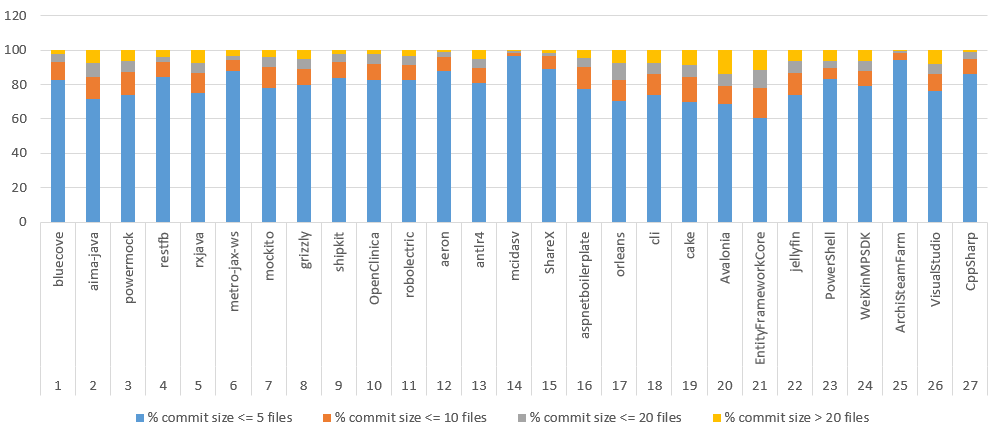
\includegraphics[width=\textwidth]{commit_distribution.png}
\caption{Commit transaction size(cs) trend in percentages.}
\label{fig:fig_cs}
\centering
\end{figure}


\begin{figure}[!h]
\centering
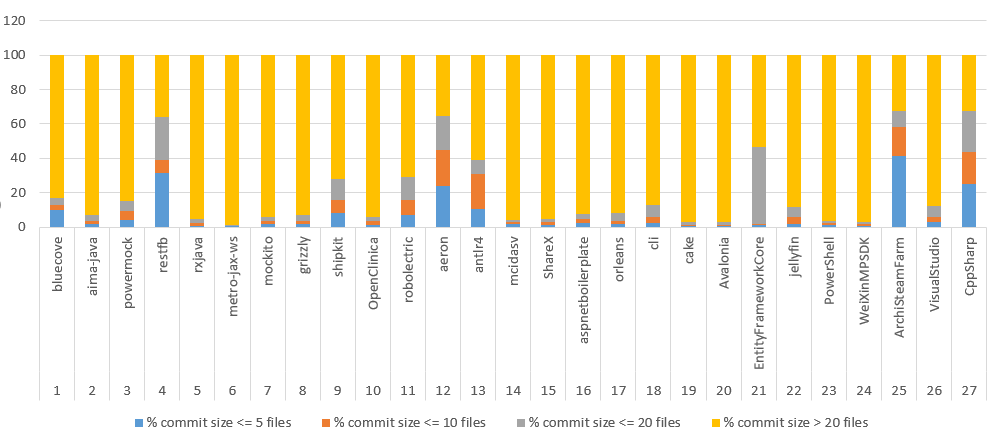
\includegraphics[width=\textwidth]{ld_distribution.png}
\caption{Percentages of LD extracted from each commit transaction size(cs) group.}
\label{fig:fig_ld_cs}
\centering
\end{figure}

As we can see in Figure \ref{fig:fig_ld_cs} even though only 5\% of the commit transactions have more than 20 files changed ($20<cs<inf$) they generate in average 80\% of the total amount of co-changing pairs extracted from the systems.
The high number of co-changing pairs extracted from such a small number of commit transactions is caused by big commit transactions. 

One single big commit transaction can lead to a large amount of logical dependencies. For example in RxJava we have commit transactions with 1030 source code files, this means that those files can generate 
$\Comb{n}{k}=\frac{n!}{k!(n-k)!} = \frac{1030!}{2!(1028)!} = 529 935$ logical dependencies. By setting a threshold on the commit transaction size we can avoid the introduction of those logical dependencies into the system.

So filtering 10\% of the total amount of commit transactions can lead to a significant decrease of the amount of logical dependencies and that is why we choose the value of 10 files as our fixed threshold for the maximum size of a commit transaction \cite{DepSACI}.



\begin{table}[!h]
\renewcommand{\arraystretch}{1}
\caption{Commit transaction size(cs) trend and average per system.}
\label{table:cs_values}
\centering
\scalebox{0.9}{
\begin{tabular}{|c|c|c|c|c|c|c|}
\hline
Nr.	  & Project    &	$cs\leq 5$	&	$cs\leq 10$	&	$cs\leq 20$	&	$cs<\infty$ & Avg	\\ 
\hline
1	&	bluecove	&	738	&	97	&	37	&	22	&	4.9	\\
2	&	aima-java	&	733	&	134	&	74	&	65	&	7.24	\\
3	&	powermock	&	685	&	128	&	66	&	70	&	9.61	\\
4	&	restfb	&	1160	&	127	&	44	&	60	&	9.9	\\
5	&	rxjava	&	3395	&	447	&	253	&	303	&	8.46	\\
6	&	metro-jax-ws	&	2583	&	198	&	78	&	68	&	4.33	\\
7	&	mockito	&	2522	&	433	&	222	&	153	&	6.33	\\
8	&	grizzly	&	2487	&	302	&	180	&	144	&	5.28	\\
9	&	shipkit	&	1311	&	151	&	64	&	37	&	4.26	\\
10	&	OpenClinica	&	2837	&	250	&	119	&	70	&	3.31	\\
11	&	robolectric	&	4827	&	503	&	264	&	318	&	7.43	\\
12	&	aeron	&	4844	&	684	&	300	&	149	&	4.6	\\
13	&	antlr4	&	3426	&	437	&	304	&	264	&	8.5	\\
14	&	mcidasv	&	3996	&	81	&	35	&	24	&	2.47	\\
15	&	ShareX	&	4731	&	529	&	145	&	80	&	4.69	\\
16	&	aspnetboilerplate	&	3208	&	569	&	321	&	225	&	6.61	\\
17	&	orleans	&	2780	&	518	&	369	&	328	&	8.95	\\
18	&	cli	&	3377	&	551	&	308	&	252	&	6.43	\\
19	&	cake	&	1785	&	359	&	174	&	200	&	9.89	\\
20	&	Avalonia	&	3806	&	641	&	371	&	446	&	8.43	\\
21	&	EntityFrameworkCore	&	2866	&	878	&	644	&	822	&	15.38	\\
22	&	jellyfin	&	4007	&	662	&	419	&	345	&	6.25	\\
23	&	PowerShell	&	2702	&	224	&	133	&	191	&	7.33	\\
24	&	WeiXinMPSDK	&	4604	&	526	&	296	&	303	&	9.01	\\
25	&	ArchiSteamFarm	&	2357	&	92	&	28	&	20	&	2.24	\\
26	&	VisualStudio	&	3902	&	521	&	295	&	321	&	6.71	\\
27	&	CppSharp	&	3870	&	390	&	203	&	59	&	3.28	\\
\hline
\end{tabular}
}
\end{table}





\section{Filtering based on number of occurrences}
\label{sec:filterocc}
One occurrence of a co-change between two software entities can be a valid logical dependency, but can also be a coincidence. Taking into consideration only co-changes with multiple occurrences as valid dependencies can lead to more accurate logical dependencies and more accurate results. On the other hand, if the project studied has a relatively small amount of commits, the probability to find multiple updates of the same classes in the same time can be small, so filtering after the number of occurrences can lead to filtering all the logical dependencies extracted. Giving the fact that we will study multiple projects of different sizes and number of commits, we will analyze also the impact of this filtering on different projects.

We have performed a series of analysis on the test systems, incrementing the threshold value occ from 1 to 4. In each of the cases the extracted logical dependencies from commit transaction with less or equal to 10 changed source code files were also filtered by the minimum number of occurrences established and all the logical dependencies that did not exceeded the minimum number of occurrences were discarded. 

The results of the analysis are presented in Table \ref{table:sd_percentages} as percentages of logical dependencies (LD) that are also structural dependencies and Table \ref{table:ld_ratio} as ratio of the number of logical dependencies (LD) to the number of structural dependencies (SD).



\begin{table}[!h]
\renewcommand{\arraystretch}{1}
\caption{Percentage of LD that are also SD}
\label{table:sd_percentages}
\centering
\scalebox{0.9}{
\begin{tabular}{|c|c|c|c|c|}
\hline
    ID  & $occ\geq 1$ & $occ\geq 2$ & $occ\geq 3$ & $occ\geq 4$  \\
\hline
1	&	7,13	&	7,77	&	7,99	&	19,71	\\
2	&	19,54	&	25,76	&	29,55	&	32,16	\\
3	&	6,66	&	8,58	&	11,82	&	14,87	\\
4	&	1,16	&	1,17	&	0,91	&	0,80	\\
5	&	3,99	&	3,96	&	7,75	&	7,49	\\
6	&	13,92	&	20,16	&	22,91	&	22,77	\\
7	&	8,38	&	9,28	&	14,93	&	14,58	\\
8	&	6,70	&	9,73	&	14,20	&	15,60	\\
9	&	16,98	&	23,34	&	29,22	&	32,89	\\
10	&	8,94	&	9,15	&	11,05	&	10,59	\\
11	&	4,99	&	6,92	&	8,88	&	11,08	\\
12	&	13,19	&	17,15	&	18,60	&	19,57	\\
13	&	2,43	&	5,59	&	8,33	&	8,21	\\
14	&	13,27	&	18,88	&	19,02	&	19,28	\\
15	&	12,90	&	21,95	&	25,51	&	27,01	\\
16	&	13,33	&	17,34	&	18,53	&	16,24	\\
17	&	6,09	&	6,18	&	6,41	&	6,44	\\
18	&	9,73	&	10,60	&	14,27	&	18,80	\\
19	&	10,26	&	13,54	&	13,64	&	12,60	\\
20	&	12,83	&	18,36	&	21,00	&	25,72	\\
21	&	2,86	&	4,65	&	5,70	&	4,98	\\
22	&	5,20	&	6,56	&	8,18	&	8,90	\\
23	&	8,23	&	13,64	&	17,04	&	17,65	\\
24	&	6,77	&	10,89	&	14,47	&	16,05	\\
25	&	9,85	&	10,15	&	11,65	&	11,33	\\
26	&	8,65	&	10,79	&	12,78	&	14,34	\\
27	&	7,04	&	8,78	&	9,87	&	10,08	\\
\hline
Avg	&	8,93	&	11,88	&	14,23	&	15,55	\\
\hline
\end{tabular}
}
\end{table}


\begin{table}[!h]
\renewcommand{\arraystretch}{1}
\caption{Ratio of number of LD to number of SD}
\label{table:ld_ratio}
\centering
\scalebox{0.9}{
\begin{tabular}{|c|c|c|c|c|}
\hline
    ID  & $occ\geq 1$ & $occ\geq 2$ & $occ\geq 3$ & $occ\geq 4$  \\
\hline
1	&	4,13	&	1,94	&	1,23	&	0,26	\\
2	&	0,81	&	0,33	&	0,16	&	0,10	\\
3	&	5,12	&	1,93	&	0,78	&	0,38	\\
4	&	53,36	&	42,00	&	38,31	&	36,30	\\
5	&	4,27	&	2,90	&	0,88	&	0,72	\\
6	&	1,07	&	0,46	&	0,30	&	0,23	\\
7	&	4,09	&	2,38	&	0,99	&	0,73	\\
8	&	4,06	&	1,57	&	0,76	&	0,49	\\
9	&	3,64	&	2,03	&	1,14	&	0,77	\\
10	&	1,41	&	1,01	&	0,47	&	0,34	\\
11	&	7,91	&	4,47	&	2,93	&	2,03	\\
12	&	3,92	&	2,15	&	1,47	&	1,07	\\
13	&	10,15	&	3,18	&	1,22	&	1,03	\\
14	&	3,07	&	1,53	&	1,16	&	0,97	\\
15	&	2,34	&	0,84	&	0,48	&	0,33	\\
16	&	1,21	&	0,47	&	0,26	&	0,19	\\
17	&	2,99	&	1,83	&	1,11	&	0,84	\\
18	&	2,26	&	1,37	&	0,67	&	0,40	\\
19	&	2,32	&	1,38	&	0,76	&	0,67	\\
20	&	1,24	&	0,58	&	0,35	&	0,18	\\
21	&	5,33	&	2,12	&	1,27	&	1,05	\\
22	&	3,38	&	1,88	&	0,99	&	0,74	\\
23	&	3,62	&	1,22	&	0,76	&	0,37	\\
24	&	2,57	&	1,22	&	0,67	&	0,46	\\
25	&	7,47	&	5,36	&	4,16	&	3,73	\\
26	&	4,03	&	2,16	&	1,50	&	1,15	\\
27	&	7,46	&	4,26	&	2,99	&	2,43	\\
\hline
Avg	&	5,67	&	3,43	&	2,51	&	2,15	\\
\hline
\end{tabular}
}
\end{table}




Based on Table \ref{table:sd_percentages} we can say that only a small percentage of the extracted logical dependencies are also structural dependencies. This is consistent with the findings of related works \cite{DBLP:journals/jss/AjienkaC17}, \cite{DBLP:journals/ese/AjienkaCC18}. The percentage of LD which are also SD  increases with the minimum number of occurrences because the number of logical dependencies from the systems decreases with the minimum number of occurrences. 
We calculate the overlapping between logical and structural dependencies not only because we want to get an idea of how many structural dependencies are reflected in the versioning system through logical dependencies but also because we want to eliminate logical dependencies that are also structural dependencies since they don't bring any new information to the systems.

We stopped the minimum occurrences threshold to 4 because we observed that for systems with ID 2, 6, 10 and 16 from Table \ref{table:ld_ratio} the ratio number is lower than 1 which means that the number of SD is higher than the number of LD. On the other hand for systems with ID 4, 11, 25, 27 the threshold of 4 for minimum number of occurrences does not change the discrepancy between the number of logical and structural dependencies.
If we try to go higher with the occurrences threshold we will risk to filter all the existing logical dependencies for some of the systems.
So, filtering with a threshold of 4 for the minimum number of occurrences will indeed filter the logical dependencies but for some of the systems the remaining number of logical dependencies will still be significantly higher compared to the number of structural dependencies.




\section{Filtering based on connection strenght}
\label{sec:filterstrength}





\section{Overlaps between structural and logical dependencies}
\label{sec:overlaps}
A logical dependency can be also a structural dependency and vice-versa, so studying the overlapping between logical and structural dependencies while filtering is important since the intention is to introduce those logical dependencies among with structural dependencies in architectural reconstruction systems. Current studies have shown a relatively small percentage of overlapping between them with and without any kind of filtering \cite{DBLP:journals/jss/AjienkaC17}. This means that a lot of non related entities update together in the versioning system, the goal here is to establish the factors that determine such a small percentage of overlapping \cite{enase19}.


In the main series of experiments, for each system, we extracted the structural dependencies and the logical dependencies and determined the overlap between the two dependencies sets, in various experimental conditions. 

One variable experimental condition is whether changes located in comments contribute towards logical dependencies. This condition distinguishes between two different cases: 
\begin{itemize}
	\item with comments: a change in source code files is counted towards a logical dependency, even if the change is inside comments in all files
	\item without comments: commits that changed source code files only by editing comments are ignored as logical dependencies
\end{itemize}

In all cases, we varied the following threshold values: 
 \begin{itemize}
	\item commit size ($cs$): the maximum size of commit transactions which are accepted to generate logical dependencies. The values for this threshold were 5, 10, 20 and no threshold (infinity).  
	\item number of occurrences ($occ$): the minimum number of repeated occurrences for a co-change to be counted as logical dependency. The values for this threshold were 1, 2, 3 and 4.  
\end{itemize}

The six tables below present the synthesis of our experiments. 
We have computed the following  values:
\begin{itemize}
	\item the mean ratio of the number of logical dependencies  (LD) to the number of structural dependencies (SD)
   \item the mean percentage of structural dependencies that are also logical dependencies (calculated from the number of overlaps divided to the number of structural dependencies)	
		\item the mean percentage of logical dependencies that are also structural dependencies (calculated from the number of overlaps divided to the number of logical dependencies)
\end{itemize}

In all the six tables, \ref{tab:ratio:comm}, \ref{tab:ratio:nocomm}, \ref{tab:percSD:comm}, \ref{tab:percSD:nocomm},
\ref{tab:percLD:comm}, \ref{tab:percLD:nocomm} we have on columns the values used for the commit size $cs$, while on rows we have the values for the number of occurrences threshold $occ$. The tables contain median values obtained for experiments done under all combinations of the two threshold values, on all test systems. In all tables, the upper right corner corresponds to the most relaxed filtering conditions, while the lower left corner corresponds to the most restrictive filtering conditions.

\begin{table}[!h]
%% increase table row spacing, adjust to taste
\renewcommand{\arraystretch}{1}
\caption{Ratio of number of LD to number of SD, case with comments}
\label{tab:ratio:comm}
\centering

\begin{tabular}{|c|c|c|c|c|}
\hline
	      &	$cs\leq 5$	&	$cs\leq 10$	&	$cs\leq 20$	&	$cs<\infty$	\\
\hline
$occ\geq 1$	&	3,39	&	5,67	&	9,00	&	80,31	\\
$occ\geq 2$	&	2,24	&	3,47	&	5,02	&	60,14	\\
$occ\geq 3$	&	1,04	&	2,53	&	3,52	&	44,68	\\
$occ\geq 4$	&	0,90	&	2,16	&	2,88	&	33,47	\\
\hline
\end{tabular}
\end{table}

\begin{table}[!h]
%% increase table row spacing, adjust to taste
\renewcommand{\arraystretch}{1}
\caption{Ratio of number of LD to number of SD, case without comments}
\label{tab:ratio:nocomm}
\centering

\begin{tabular}{|c|c|c|c|c|}
\hline
	      &	$cs\leq 5$	&	$cs\leq 10$	&	$cs\leq 20$	&	$cs< \infty$	\\
\hline
$occ\geq 1$	&	3,24	&	5,33	&	7,90	&	67,16	\\
$occ\geq 2$	&	1,35	&	3,27	&	4,72	&	47,39	\\
$occ\geq 3$	&	1,00	&	1,67	&	2,49	&	32,39	\\
$occ\geq 4$	&	0,43	&	1,26	&	1,93	&	22,15	\\
\hline
\end{tabular}
\end{table}

\begin{table}[!h]
%% increase table row spacing, adjust to taste
\renewcommand{\arraystretch}{1}
\caption{Percentage of SD that are also LD, case with comments}
\label{tab:percSD:comm}
\centering

\begin{tabular}{|c|c|c|c|c|}
\hline
	      &	$cs\leq 5$	&	$cs\leq 10$	&	$cs\leq 20$	&	$cs< \infty$	\\
\hline
$occ\geq 1$	&	19,75	&	29,86	&	39,29	&	76,59	\\
$occ\geq 2$	&	12,50	&	20,20	&	27,68	&	66,11	\\
$occ\geq 3$	&	8,49	&	14,22	&	19,94	&	55,99	\\
$occ\geq 4$	&	6,58	&	10,95	&	15,76	&	47,12	\\
\hline
\end{tabular}
\end{table}

\begin{table}[!h]
%% increase table row spacing, adjust to taste
\renewcommand{\arraystretch}{1}
\caption{Percentage of SD that are also LD, case without comments}
\label{tab:percSD:nocomm}
\centering

\begin{tabular}{|c|c|c|c|c|}
\hline
	      &	$cs\leq 5$	&	$cs\leq 10$	&	$cs\leq 20$	&	$cs< \infty$	\\
\hline
$occ\geq 1$	&	18,88	&	28,47	&	37,44	&	71,12	\\
$occ\geq 2$	&	11,87	&	19,03	&	25,93	&	59,58	\\
$occ\geq 3$	&	8,00	&	13,09	&	18,15	&	48,65	\\
$occ\geq 4$	&	5,85	&	9,94	&	14,27	&	39,07	\\
\hline
\end{tabular}
\end{table}

\begin{table}[!h]
%% increase table row spacing, adjust to taste
\renewcommand{\arraystretch}{1}
\caption{Percentage of LD that are also SD, case with comments}
\label{tab:percLD:comm}
\centering

\begin{tabular}{|c|c|c|c|c|}
\hline
	      &	$cs\leq 5$	&	$cs\leq 10$	&	$cs\leq 20$	&	$cs< \infty$	\\
\hline
$occ\geq 1$	&	12,02	&	8,86	&	6,72	&	1,79	\\
$occ\geq 2$	&	15,05	&	11,71	&	9,38	&	2,21	\\
$occ\geq 3$	&	17,45	&	13,97	&	11,57	&	2,86	\\
$occ\geq 4$	&	18,96	&	15,28	&	12,94	&	3,67	\\
\hline
\end{tabular}
\end{table}

\begin{table}[!h]
%% increase table row spacing, adjust to taste
\renewcommand{\arraystretch}{1}
\caption{Percentage of LD that are also SD, case without comments}
\label{tab:percLD:nocomm}
\centering
\begin{tabular}{|c|c|c|c|c|}
\hline
	      &	$cs\leq 5$	&	$cs\leq 10$	&	$cs\leq 20$	&	$cs< \infty$	\\
\hline
$occ\geq 1$	&	12,05	&	9,02	&	6,98	&	1,93	\\
$occ\geq 2$	&	15,08	&	12,03	&	9,66	&	2,42	\\
$occ\geq 3$	&	17,78	&	14,37	&	12,24	&	3,28	\\
$occ\geq 4$	&	19,22	&	15,59	&	13,30	&	4,21	\\
\hline
\end{tabular}
\end{table}

In order to assess the influence of comments, we compare pairwise Tables \ref{tab:ratio:comm} and \ref{tab:ratio:nocomm},  
Tables \ref{tab:percSD:comm} and \ref{tab:percSD:nocomm} and Tables \ref{tab:percLD:comm} and \ref{tab:percLD:nocomm}. 
We observe that, although there are some differences between pairs of measurements done in similar conditions with and without comments, the differences are not significant.

On the other hand, the overlap between structural and logical dependencies is given by the number of pairs of classes that have both structural and logical dependencies. We evaluate this overlap as a percentage relative to the number of structural dependencies in Tables \ref{tab:percSD:comm} and \ref{tab:percSD:nocomm}, respectively as  a percentage relative to the number of logical dependencies in Tables \ref{tab:percLD:comm} and \ref{tab:percLD:nocomm}.

A first observation from Tables \ref{tab:percSD:comm} and \ref{tab:percSD:nocomm} is that not all pairs of classes with structural dependencies co-change. The biggest value for the percentage of structural dependencies that are also logical dependencies is 76.5\% obtained in the case when no filterings are done.

From Tables \ref{tab:percLD:comm} and \ref{tab:percLD:nocomm} we notice that the percentage of logical dependencies which are also structural is always low to very low. This means that most co-changes are recorded between classes that have no structural dependencies to each other \cite{enase19}.   
 

\chapter{Conclusions}
\label{conclusions}

 %%%%%%%%%%%%%%%%%%%%%%%%%%%%%%%%%%%%%%%%%%%%%%%%%%%%%%%%%%%%%%%%%%%%%%%%%%%%%%%%


\bibliographystyle{plain}
\bibliography{logicaldepd}
\end{document}

